\subsection{准素子模}

命题 1. 设 A 是诺特环，M 是 A-模。下列条件等价：(a) Ass(M) 归结为单个元素。

\begin{enumerate}
\def\labelenumi{(\alph{enumi})}
\setcounter{enumi}{1}
\tightlist
\item
  \(\mathbf{M} \neq 0\)，且 \(\mathbf{M}\) 的每个伸缩映射或者是单射，或者是殆幂零的（§ 1，第 4 节）。若这些条件满足，且 \(\mathfrak{p}\) 是所有使伸缩映射 \(a \in \mathbf{A}\) 殆幂零的 \(a_{\mathbf{M}}\) 所成的集合，则 \(\operatorname{Ass}(\mathbf{M}) = \{\mathfrak{p}\}\)。
\end{enumerate}

这立即由 § 1，第 4 节，命题 9 的推论以及第 1 节命题 2 的推论 2 得出。

定义 1. 设 A 是诺特环，N 是 A-模，Q 是 N 的子模。如果模 M = N/Q 满足命题 1 的条件，则称 Q 关于 N（或在 N 中）是 p-准素的。

在没有歧义时，我们简称 Q 为“p-准素的”或“准素的”；显然，对于 N 中包含 Q 的每个子模 \(N' \neq Q\)，Q 在 \(N'\) 中都是 p-准素的。

定义 1 特别适用于 N = A 的情形；此时 N 的子模就是 A 的理想，因此 A 的理想 q 称为准素理想，如果 Ass(A/q) 归结为单个元素，或者等价地，如果 A ≠ q 且环 A/q 中的每个零因子都是幂零的。如果 q 是 p-准素的，则由定义 1，p 是理想 q 的根（第二章，第 2 节，第 6 节）。

注。设 q 是 A-模 N 的 p-准素子模。如果 N/Q 是有限生成的，则由第 1 节，命题 9，存在整数 k \textgreater{} 0，使得 \(p^{k}N \subset Q\)。

\textbf{例}\par

\begin{enumerate}
\def\labelenumi{(\arabic{enumi})}
\item
  如果 \(\mathfrak{p}\) 是 \(\mathbf{A}\) 的素理想，则 \(\mathfrak{p}\) 是 \(\mathfrak{p}\)-准素的（§ 1，第 1 节，命题 1）。
\item
  设 q 是 A 的理想，且存在唯一一个包含 q 的素理想 m（必然是极大理想）；那么，如果 M 是满足 \(qM \neq M\) 的 A-模，qM 关于 M 是 m-准素的。因为 \(\text{Ass}(M/qM)\) 中的每个元素都包含 q，故都等于 m，且 \(\text{Ass}(M/qM) \neq \varnothing\)（§1，第 1 节，命题 2 的推论 1）。特别地，q 是 A 中的 m-准素理想。
\item
  设 \(\mathfrak{m}\) 是 \(\mathbf{A}\) 的极大理想；\(\mathfrak{m}\)-准素理想正是 \(\mathfrak{q}\) 的理想 \(\mathbf{A}\)，对于这些理想，存在整数 \(n \geqslant 1\)，使得 \(\mathfrak{m}^n \subset \mathfrak{q} \subset \mathfrak{m}\)。因为若 \(\mathfrak{m}^n \subset \mathfrak{q} \subset \mathfrak{m}\)，\(\mathfrak{m}\) 是包含 \(\mathfrak{q}\) 的唯一素理想（第二章，第 1 节，第 1 节，命题 1 的推论），结论由例 2 得出；反之，若 \(\mathfrak{q}\) 是 \(\mathfrak{m}\)-准素的，则 \(\mathfrak{m}\) 是 \(\mathfrak{q}\) 的根，因此存在 \(n \geqslant 1\)，使得 \(\mathfrak{m}^n \subset \mathfrak{q}\)（第二章，第 2 节，第 6 节，命题 15）。
\item
  在主理想整环 A 中，准素理想是 (0) 以及形如 \(Ap^{n}\) 的理想，其中 p 是极端元且 \(n \geqslant 1\)；这立即由例 3 得出。
\end{enumerate}

% \pandocbounded{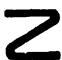
\includegraphics[keepaspectratio]{images/part002_84c4f053.jpg}}


\begin{enumerate}
\def\labelenumi{(\arabic{enumi})}
\setcounter{enumi}{4}
\tightlist
\item
任一素理想的幂不一定是准素理想（习题 1）。另一方面，存在不是素理想幂的准素理想（习题 1）。
\end{enumerate}

命题 2. 设 M 是诺特环上的模，p 是 A 的素理想，\((Q_{i})_{i\in I}\) 是 M 的非空有限子模族，且这些子模关于 M 都是 p-准素的。则 \(\bigcap_{i\in I} Q_{i}\) 关于 M 是 p-准素的。

\(\mathrm{M}/\left(\bigcap_{i\in\mathrm{I}}\mathrm{Q}_{i}\right)\) 同构于一个 \(\neq0\) 的子模，它是直和 \(\bigoplus_{i\in\mathrm{I}}(\mathrm{M}/\mathrm{Q}_{i})\) 的子模。现在

\[
\operatorname{Ass} \left(\bigoplus_ {i \in I} (M / Q _ {i})\right) = \bigcup_ {i \in I} \operatorname{Ass} (M / Q _ {i}) = \{p \}
\]

（§ 1，第 1 节，命题 3 的推论 1）。因此 \(\operatorname{Ass}\left(M / \left(\bigcap_{i \in I} Q_i\right)\right) = \{p\}\)（§ 1，第 1 节，命题 3 及命题 2 的推论 1）。

命题 3. 设 A 是诺特环，S 是 A 的乘性子集，p 是 A 的素理想，M 是 A-模，N 是 M 的子模，且 \(i = i_{A}^{S}\) 是从 M 到 \(S^{-1}M\) 的典范映射。

\begin{enumerate}
\def\labelenumi{(\roman{enumi})}
\item
  假设 \(\mathfrak{p} \cap \mathbf{S} \neq \varnothing\)。若 \(\mathbf{N}\) 关于 \(\mathfrak{p}\) 是 \(\mathbf{M}\)-准素的，则 \(\mathbf{S}^{-1}\mathbf{N} = \mathbf{S}^{-1}\mathbf{M}\)。
\item
  假设 \(\mathfrak{p} \cap \mathbf{S} = \varnothing\)。要使 \(\mathbf{N}\) 关于 \(\mathfrak{p}\) 是 \(\mathbf{M}\)-准素的，充要条件是 \(\mathbf{N}\) 具有 \(i^{-1}(\mathbf{N}')\) 的形式，其中 \(\mathbf{N}'\) 是 \(\mathbf{S}^{-1}\mathbf{A}\)-子模，且是 \(\mathbf{S}^{-1}\mathbf{M}\) 的子模，并且关于 \((\mathbf{S}^{-1}\mathfrak{p})\) 是 \(\mathbf{S}^{-1}\mathbf{M}\)-准素的；此时 \(\mathbf{N}' = \mathbf{S}^{-1}\mathbf{N}\)。
\item
  如果 \(\mathfrak{p} \cap S \neq \varnothing\)，且 \(N\) 关于 \(\mathfrak{p}\) 是 \(M\)-准素的，则
\end{enumerate}

\[
\mathrm{Ass} _ {\mathbf {S} ^ {- 1} \mathbf {A}} (\mathrm{S} ^ {- 1} (\mathrm{M} / \mathrm{N})) = \varnothing
\]

（§ 1，第 2 节，命题 5 的推论），因此 \(S^{-1}(M/N) = 0\)（§ 1，第 1 节，命题 2 的推论 1），从而 \(S^{-1}M/S^{-1}N = 0\)。

\begin{enumerate}
\def\labelenumi{(\roman{enumi})}
\setcounter{enumi}{1}
\tightlist
\item
   假设\(\mathfrak{p} \cap \mathrm{S} = \varnothing\)。若\(\mathbf{N}\)是\(\mathfrak{p}\)-准素的（相对于\(\mathbf{M}\)），则\(\operatorname{Ass}_{\mathbf{S}^{-1}\mathbf{A}}(\mathrm{S}^{-1}(\mathrm{M/N})) = \{\mathrm{S}^{-1}\mathfrak{p}\}\)（\(\S 1\)，第 2 节，命题 5 的推论）因此，子模\(\mathbf{N}' = \mathrm{S}^{-1}\mathbf{N}\)的\(\mathrm{S}^{-1}\mathbf{M}\)是\((\mathrm{S}^{-1}\mathfrak{p})\)-准素的；此外，若\(s \in \mathbf{S}\)和\(m \in \mathbf{M}\)满足\(sm \in \mathbf{N}\)，则\(m \in \mathbf{N}\)，因为在\(s\)中比为\(\mathbf{M/N}\)的伸缩映射是单射，从而\(\mathbf{N} = \overline{i}^{1}(\mathbf{N}')\)（第二章，\(\S 2\)，第 4 节，命题 10）。反之，设\(\mathbf{N}'\)是\(\mathrm{S}^{-1}\mathbf{M}\)的子模，它是\((\mathrm{S}^{-1}\mathfrak{p})\)-准素的（相对于\(\mathrm{S}^{-1}\mathbf{M}\)）；记\(\mathbf{N} = \overline{i}^{1}(\mathbf{N}')\)；则\(\mathbf{N}' = \mathrm{S}^{-1}\mathbf{N}\)（第二章，\(\S 2\)，第 4 节，命题 10），并且\(\operatorname{Ass}_{\mathbf{S}^{-1}\mathbf{A}}(\mathrm{S}^{-1}(\mathrm{M/N})) = \operatorname{Ass}_{\mathbf{S}^{-1}\mathbf{A}}((\mathrm{S}^{-1}\mathbf{M})/\mathrm{N}') = \{\mathrm{S}^{-1}\mathfrak{p}\}\)。由于典范映射\(\mathrm{M/N} \to \mathrm{S}^{-1}(\mathrm{M/N})\)是单射，\(\mathbf{A}\)中与\(\mathbf{M/N}\)相关联的每个素理想都不与\(\mathbf{S}\)相交（\(\S 1\)，第 2 节，命题 6）；因此\(\operatorname{Ass}(\mathrm{M/N}) = \{\mathfrak{p}\}\)（\(\S 1\)，第 2 节，命题 5 的推论），所以\(\mathbf{N}\)是\(\mathfrak{p}\)-准素的（相对于\(\mathbf{M}\)）。
\end{enumerate}

